\documentclass[./project-report/src/latex/project-report.tex]{subfiles}

\begin{document}

\maketitle

\clearpage
\section{Analysis}

\subsection{Theory Behind Artificial Neural Networks}
\label{sec:ann-theory}

From an abstract perspective, Artificial Neural Networks are inspired by the anatomy of the human brain, consisting of layers of 'neurons' all interconnected via 
different links, 'axons with connecting synapses', each with their own strengths, 'weights'. By adjusting these links and weights, Artificial Neural Networks can be trained 
to take in an input and give its best prediction as an output.

\begin{figure}[h!]
\centering
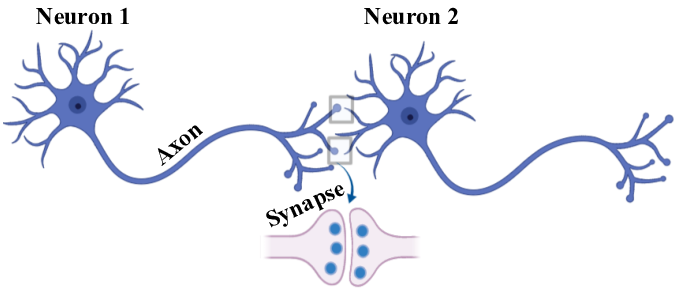
\includegraphics[width=1\textwidth]{./project-report/src/images/connected-neurons.png}
\caption{Two connected biological neurons sourced from https://www.researchgate.net}
\end{figure}

\vspace{5mm}

\subsubsection{Structure}

\begin{figure}[h!]
\centering
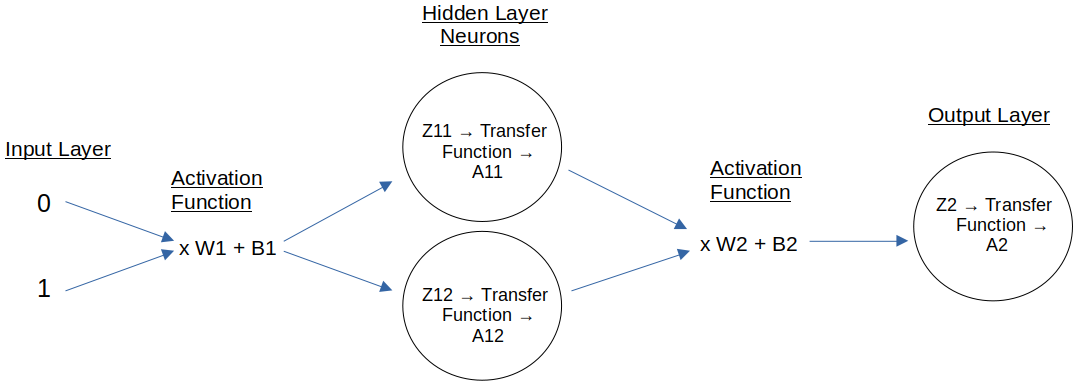
\includegraphics[width=1\textwidth]{./project-report/src/images/shallow-ann-diagram.png}
\caption{This shows an Artificial Neural Network with one single hidden layer and is known as a Shallow Neural Network.}
\end{figure}

I have focused on Feed-Forward Artificial Neural Networks, where values are entered to the input layer and passed forwards repetitively to the next layer until 
reaching the output layer. Within this, I have investigated two types of Feed-Forward Artificial Neural Networks: Perceptron Artificial Neural Networks, that contain no 
hidden layers and are suitable for addressing simple linear problems, and Multi-Layer Perceptron Artificial Neural Networks, that contain at least one hidden layer. 
The expanded complexity of the Multi-Layer Perceptron Artificial Neural Network increases the non-linearity in the Artificial Neural Network allowing it to address 
more complex / non-linear problems.

\vspace{5mm}

\noindent
Multi-Layer Perceptron Artificial Neural Networks consist of:

\begin{itemize}
    \item An input layer of input neurons, where the input values are entered.
    \item Hidden layers of hidden neurons.
    \item An output layer of output neurons, which outputs the final prediction.
\end{itemize}

To implement an Artificial Neural Network, matrices are typically used to represent the layers, where each layer is a matrix of the layer's neuron's values. In 
order to use matrices for this, the following basic theory must be known about them:

\begin{itemize}
    \item When Adding two matrices, both matrices must have the same number of rows and columns. Alternatively, a single column matrix with the same number of rows can be 
          added by element-wise addition where each element is added to all of the elements of the corresponding rows in the associated matrix.
    \item In order to multiply matrices, the 'dot product' of the matrices is computed which multiplies the rows of one matrice with the columns of the other, multiplying 
          matching members and then summing up.
    \item When calculating the dot product of two matrices, the number of columns of the 1st matrix must equal the number of rows of the 2nd matrix. The resulting matrix will 
          have the same number of rows as the 1st matrix, and the same number of columns as the 2nd matrix. This is important in implementing an Artificial Neural Network, 
          as the output of one layer must be formatted correctly to be used with the next layer.
    \item Alternatively, the Hadamard product of two matrices can be utilised which performs element-wise multiplication of the matrices. For this, both matrices 
          must have the same number of rows and columns.
    \item Transposing a matrix is also utilised which switches all rows of the matrix into columns and all columns into rows in an output matrix.
    \item A matrix of values can be classified as a rank of Tensors, depending on the number of dimensions of the matrix. (Eg: A 2-dimensional matrix is a Tensor of 
          rank 2)
\end{itemize}

I have focused on using Fully-Connected layers, that input values and apply the following functions to produce an output value for the layer:

\begin{itemize}
    \item \textbf{Activation function} which calculates the dot product of an input matrix with a weight matrix, then sums the result with a bias matrix.
    \item \textbf{Transfer function} which takes the result of the activation function and calculates a suitable output value as well as adding more non-linearity to the Neural Network. 
          For example, the Sigmoid Transfer function converts the input value to an output number between zero and one - this makes it useful for logistic regression where the output value 
          can be rounded to allow for a binary classification.
\end{itemize}

\vspace{5mm}

\subsubsection{How Artificial Neural Networks learn}
\vspace{5mm}

To train an Artificial Neural Network, the following processes are carried out for each of a number of training iterations called epochs:

\begin{itemize}
    \item Forward Propagation which is the process of feeding inputs in and getting a prediction (moving forward through the network).
    \item Back Propagation, the process of calculating the error, known as the loss, in the prediction and then adjusting the weights and biases accordingly.
\end{itemize}

I have used Supervised Learning to train the Artificial Neural Networks, where the output prediction of the Artificial Neural Network is compared to the theoretical values it should have 
predicted. With this, I can calculate the loss value of the prediction. I then move back through the network and update the weights and biases via Gradient Descent which aims to reduce 
the Loss value of the prediction to a minimum, by subtracting the rate of change of Loss with respect to the weights / biases, multiplied with a learning rate, from the weights / biases. 
To calculate the rate of change of Loss with respect to the weights / biases, I used the following calculus methods:

\begin{itemize}
    \item Partial Differentiation, which allows differentiation of multi-variable functions, by differentiating with respect to one variable and treating the rest as constants.
    \item The Chain Rule, where for $y = f(u)$ and $u = g(x)$, $\frac{\partial{y}}{\partial{x}}$ can be calculated as: $\frac{\partial{y}}{\partial{x}} = \frac{\partial{y}}{\partial{u}} * \frac{\partial{u}}{\partial{x}}$.
\end{itemize}

This repetitive process will continue to reduce the Loss to a minimum, if the learning rate is set to an appropriate value

\begin{figure}[h!]
\centering
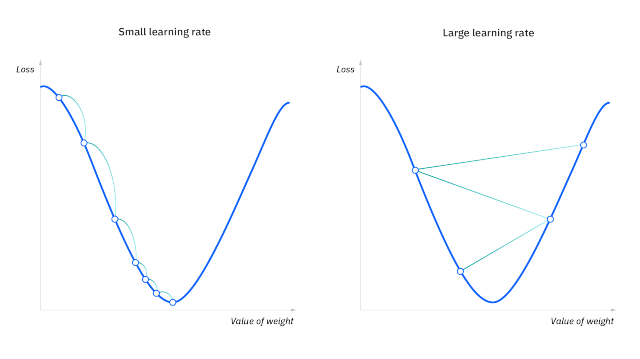
\includegraphics[width=1\textwidth]{./project-report/src/images/gradient-descent.png}
\caption{Gradient Descent\\
        sourced from https://www.ibm.com/topics/gradient-descent}
\end{figure}

\pagebreak

However, during backpropagation some issues can occur, such as the following:

\begin{itemize}
    \item Finding a false local minimum rather than the global minimum of the function
    \item Having an 'Exploding Gradient', where the gradient value grows exponentially to the point of overflow errors
    \item Having a 'Vanishing Gradient', where the gradient value decreases to a very small value or zero, resulting in a lack of updating values during training.
\end{itemize}

\pagebreak

\subsection{Theory Behind Deep Artificial Neural Networks}
\vspace{5mm}

\subsubsection{Network Architecture and Training}

\begin{figure}[h!]
\centering
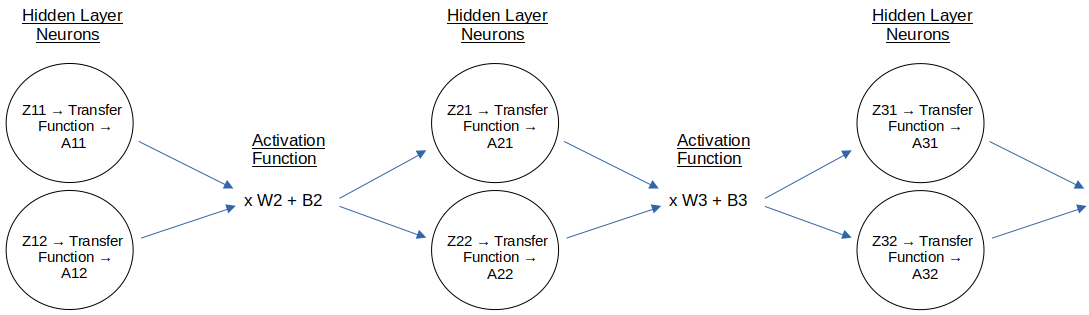
\includegraphics[width=1\textwidth]{./project-report/src/images/deep-ann-diagram-2.png}
\caption{This shows an Artificial Neural Network with multiple hidden layers and is known as a Deep Neural Network.}
\label{fig:abstract-network}
\end{figure}

Figure \ref{fig:abstract-network} below shows a simplified view of an Artificial Neural Network with multiple hidden layers, known as a Deep Neural Network, where:

\pagebreak

\begin{figure}[h!]
\centering
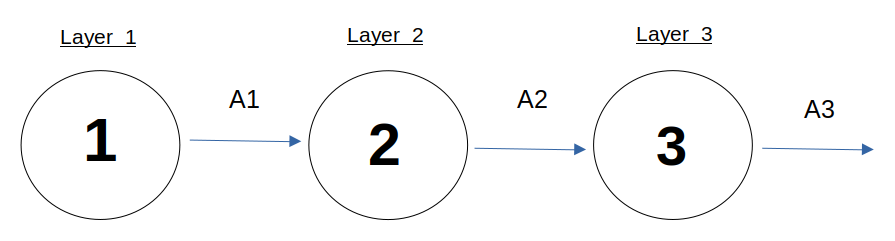
\includegraphics[width=1\textwidth]{./project-report/src/images/deep-ann-diagram.png}
\caption{Showing an abstracted view of an Artificial Neural Network with multiple hidden layers.}
\label{fig:abstract-network}
\end{figure}

\begin{itemize}
    \item Each layer takes the previous layer's output as its input X
    \item An Activation function is applied to X to obtain Z, by taking the dot product of X with a weight matrix W, and sums the result with a bias matrix B. At 
          first when the Neural Network is initialised pre-training the weights are initialised to random values and the biases are set to zeros.
          $Z = W * X + B$
    \item A Transfer function is then applied to Z to obtain the layer's output A
    \begin{itemize}
        \item For the output layer, the sigmoid function (explained previously) can be used for either for binary classification via logistic regression, or for multi-
              class classification where the output neuron, and the associated class, that has the highest value between zero and one is selected.
        \begin{itemize}
            \item Where $sigmoid(Z) = \frac{1}{1+e^{-Z}}$
        \end{itemize}
        \item However, for the input layer and the hidden layers, another transfer function known as ReLu (Rectified Linear Unit) can be better suited as it produces 
              larger values of $\frac{\partial{L}}{\partial{W}}$ and $\frac{\partial{L}}{\partial{B}}$ for Gradient Descent than Sigmoid, so updates at a quicker rate.
        \begin{itemize}
            \item Where $relu(Z) = max(0, Z)$
        \end{itemize}
    \end{itemize}
\end{itemize}

\subsubsection{Training}

Training takes place through a series of forward and backward propagation called epochs. The forward propagation generates a potential output and associated error known 
as the loss. Backward propagation then adjusts the weights and biases in an attempt to reduce this loss.

\subsubsection{Forward Propagation:}

\begin{itemize}
    \item For each epoch the input layer is presented with a matrix of input values, which are fed through the network to obtain a final prediction A from the output layer.
	\item Using the process described in the previous section, backpropagation trains the network by adjusting weights and biases.
\end{itemize}

\subsubsection{Back Propagation:}

\begin{itemize}
    \item First the Loss value L is calculated using the following Log-Loss function, which calculates the average difference between A and the value it should have 
          predicted Y. The average is then found by summing the result of the Loss function for each value in the matrix A, then dividing by the number of predictions m, 
          resulting in a Loss value indicating how well the network is performing.
    	  Where $L = -(\frac{1}{m}) * \sum(Y * log(A) + (1-Y) * log(1-A))$ and "log()" is the natural logarithm
    \item The network is then trained by moving back through the layers, adjusting the weights and biases via Gradient Descent. For each layer, the weights and biases are 
		  updated with the following formulae:
    \begin{itemize}
        \item $W = W - learningRate * \frac{\partial{L}}{\partial{W}}$
        \item $B = B - learningRate * \frac{\partial{L}}{\partial{B}}$
    \end{itemize}
    \item The derivation for Layer 2's $\frac{\partial{L}}{\partial{W}}$ and $\frac{\partial{L}}{\partial{B}}$ is shown below:
    \begin{itemize}
        \item Functions used so far:
        \begin{enumerate}
            \item $Z = W * X + B$
            \item $A_{relu} = max(0, Z)$
            \item $A_{sigmoid} = \frac{1}{1+e^{-Z}}$
            \item $L = -(\frac{1}{m}) * \sum(Y * log(A) + (1-Y) * log(1-A))$
        \end{enumerate}
        \item $\frac{\partial{L}}{\partial{A2}} = \frac{\partial{L}}{\partial{A3}} * \frac{\partial{A3}}{\partial{Z3}} * \frac{\partial{Z3}}{\partial{A2}}$
              \vspace{1mm}
              \newline
              By using function 1, where A2 is X for the 3rd layer, $\frac{\partial{Z3}}{\partial{A2}} = W3$
              \vspace{1mm}
              \newline
              $=> \frac{\partial{L}}{\partial{A2}} =  \frac{\partial{L}}{\partial{A3}} * \frac{\partial{A3}}{\partial{Z3}} * W3$
        \item $\frac{\partial{L}}{\partial{W2}} = \frac{\partial{L}}{\partial{A2}} * \frac{\partial{A2}}{\partial{Z2}} * \frac{\partial{Z2}}{\partial{W2}}$
              \vspace{1mm}
              \newline
              By using function 1, where A1 is X for the 2nd layer, $\frac{\partial{Z2}}{\partial{W2}} = A1$
              \vspace{1mm}
              \newline
              $=> \frac{\partial{L}}{\partial{W2}} = \frac{\partial{L}}{\partial{A2}} * \frac{\partial{A2}}{\partial{Z2}} * A1$
        \item $\frac{\partial{L}}{\partial{B2}} = \frac{\partial{L}}{\partial{A2}} * \frac{\partial{A2}}{\partial{Z2}} * \frac{\partial{Z2}}{\partial{B2}}$
              \vspace{1mm}
              \newline
              By using function 1, $\frac{\partial{Z2}}{\partial{B2}} = 1$
              \vspace{1mm}
              \newline
              $=> \frac{\partial{L}}{\partial{W2}} = \frac{\partial{L}}{\partial{A2}} * \frac{\partial{A2}}{\partial{Z2}} * 1$
    \end{itemize}
    \item As can be seen, when moving back through the network, $\frac{\partial{L}}{\partial{W}}$ and $\frac{\partial{L}}{\partial{B}}$ can be calculated for each layer 
		  with the rate of change of loss with respect to its output, which is calculated by the previous layer using the above formula; the derivative of 
          the layer's transfer function, and the layers input (which in this case is A1)
    \begin{itemize}
        \item Where by using function 2, $\frac{\partial{A_{relu}}}{\partial{Z}} = 1$ when $Z >= 0$ otherwise $\frac{\partial{A_{relu}}}{\partial{Z}} = 0$
        \item Where by using function 3, $\frac{\partial{A_{sigmoid}}}{\partial{Z}} = A * (1 - A)$
    \end{itemize}
    \item At the start of backpropagation, the rate of change of loss with respect to the output layer's output has no previous layer's calculations, so instead it can 
          be found with the derivative of the Log-Loss function, as shown in the following:
    \begin{itemize}
        \item Using function 4, $\frac{\partial{L}}{\partial{A}} = (-\frac{1}{m})(\frac{Y-A}{A * (1-A)})$
    \end{itemize}
\end{itemize}

\subsection{Theory behind training the Artificial Neural Networks}

Training an Artificial Neural Network's weights and biases to predict on a dataset, will create a trained model for that dataset. This model can be used to create 
predictions based on future data / images inputted. However, training Artificial Neural Networks involves problems such as Overfitting, where the trained model learns 
the patterns of the training dataset too well, resuting in poor predictions on new datasets. This can occur when the training dataset does not cover enough situations 
of inputs and the desired outputs (by being too small for example), if the model is trained for too many epochs on the poor dataset or by having too many layers in the 
Neural Network.

Another common problem is Underfitting, where the model has not learnt the patterns of the training dataset well enough, often when it has been trained for too few 
epochs, or when the Neural Network is too linear.

\subsubsection{Datasets}

I have utilised a series of open source datasets on which to train and test by Neural Networks.

\subsubsection{XOR dataset}

As a first step in developing and testing Artificial Neural Networks, I have utilised the XOR gate problem, where the Neural Network is fed input pairs of zeros and 
ones and learns  to predict the output of a XOR gate used in circuits. This takes far less computation time than image datasets and is extremely useful in debugging. 
It is a good example of a relatively simple problem whilst not being linearly separable.

\subsubsection{MNIST dataset}

The MNIST dataset is a well known dataset consisting of images of handwritten digits from zero to ten and is commonly used to test the performance of an Artificial Neural 
Network. The dataset consists of 60,000 input images representing single digits made up from 28x28 pixels with each pixel having an RGB value from 0 to 255. To format the 
images into a suitable format to be inputted into the Artificial Neural Networks, each image's matrix of RGB values is commonly 'flattened' into a 1 dimensional matrix of 
values, where each element is also divided by 255 (the max RGB value) to produce a number between 0 and 1, to standardize the dataset. The output dataset is also loaded which 
represents the actual value of the number in the image. This is commonly implemented by using an array for each image where the index of the array represesents the number in 
an image (i.e. a 1 in column 2 could represent a 2, or a 1 if zero indexed).

To create a trained Artificial Neural Network model on this dataset, the model requires 10 output neurons (one for each digit). The Sigmoid Transfer function is then utilized 
to output a number between one and zero to each neuron - whichever neuron received the highest value is selected as the predicted outcome. This an example of a multi-class 

classification, where the model must predict one of 10 classes (in this case, each class is one of the digits from zero to ten).
\subsubsection{Cat dataset}

I have also used a dataset of images of cats sourced from https://github.com/marcopeix, where each image is classified as either a cat or not a cat. The dataset consists of 
209 input images, made up from 64x64 pixels with each pixel having an RGB value from 0 to 255. To normalise the images into a suitable format to be input into the Artificial 
Neural Network, each image's matrix of RGB values is 'flattened' into a 1 dimensional matrix of values, where each element is divided by 255 (the max RGB value) to a number 
between 0 and 1, to standardize the dataset.

The output dataset represents an array of binary values representing the output of each image (1 for a cat, 0 for not a cat). To create a trained Artificial Neural Network model 
on this dataset, the model requires only 1 output neuron - representing the chance of being a cat. By using the Sigmoid Transfer function, a number is outputted between one and zero 
for the neuron, if the neuron's value is closer to 1 it predicts a cat, otherwise it predicts not a cat - this is binary classification.

\subsubsection{Theory behind using Graphics Cards to train Artificial Neural Networks}
\vspace{5mm}

Graphics Cards have been designed essentially to undertake parallel matrix computations utilising many Tensor cores - which are processing units specialised for matrix operations 
calculating the co-ordinates of 3D graphics, however they can be used for operating on the matrices in the network at a much faster speed compared to CPUs. GPUs also include CUDA 
cores which act as an API to the GPU's computing to be used for any operations (in this case training the Artificial Neural Networks).

\subsection{Interview}

In order to gain a better foundation for my investigation, and ensure my project would allow a user interested in Artificial Neural Networks to experiment with the 
fundamentals of the network and conduct experiments, I presented my prototype code and interviewed the head of Artificial Intelligence at Cambridge Consultants. 
These were their responses:

\begin{itemize}
    \item Q:"Are there any good resources you would recommend for learning the theory behind how Artificial Neural Networks work?"
    
          A:"There are lots of useful free resources on the internet to use. I particularly like the platform 'Medium' which offers many scientific articles 
             as well as more obvious resources such as IBMs'."
    \item Q:"What do you think would be a good goal for my project?"

          A:"I think it would be great to aim for applying the Neural Networks on Image Recognition for some famous datasets. For you, I would recommend 
             the MNIST dataset as a goal."
    \item Q:"What features of the Artificial Neural Networks would you like to be able to experiment with?"

          A:"I'd like to be able to experiment with the number of layers and the number of neurons in each layer, and then be able to see how these changes effect 
             the performance of the model. I can see that you've utilised the Sigmoid transfer function and I would recommend having the option to test alternatives 
              such as the ReLu transfer function, which will help stop issues such as a vanishing gradient."
    \item Q:"What are some practical constraints of AI?"

          A:"Training AI models can require a large amount of computing power, also large datasets are needed for training models to a high accuracy which can be hard 
             to obtain."
    \item Q:"What would you say increases the computing power required the most?"

          A:"The number of layers and neurons in each layer will have the greatest effect on the computing power required. This is another reason why I recommend adding 
             the ReLu transfer function as it updates the values of the weights and biases faster than the Sigmoid transfer function."
    \item Q:"Do you think I should explore other computer architectures for training the models?"

          A:"Yes, it would be great to add support for using graphics cards for training models, as this would be a vast improvement in training time compared to using 
             just CPU power."
    \item Q:"I am also creating a user interface for the program, what hyper-parameters would you like to be able to control through this?"

          A:"It would be nice to control the transfer functions used, as well as the general hyper-parameters of the model. I also think you could add a progress tracker 
             to be displayed during training for the user."
    \item Q:"How do you think I should measure the performance of models?"

          A:"You should show the accuracy of the model's predictions, as well as example incorrect and correct prediction results for the trained model. Additionally, 
             you could compare how the size of the training dataset effects the performance of the model after training, to see if a larger dataset would seem 
             beneficial."
    \item Q:"Are there any other features you would like add?"

          A:"Yes, it would be nice to be able to save a model after training and have the option to load in a trained model for testing."
\end{itemize}

Based on the interview above, the following high-level objectives were formulated:

\subsection{Project Objectives}

\begin{tabular}{|p{0.13\linewidth}|p{0.87\linewidth}|}
      \hline
      \textbf{Objective ID} & \textbf{Description} \\
      \hline
      1 & Learn how Artificial Neural Networks work and develop them from first principles \\
      \hline
      2 & Implement the Artificial Neural Networks by creating trained models based on image datasets \\
      \hline
      2.1 & Allow use of Graphics Cards for faster training \\
      \hline
      2.2 & Allow for the saving and loading of trained models \\
      \hline
      3 & Develop a Graphical User Interface \\
      \hline
      3.1 & Provide controls for hyper-parameters of models \\
      \hline
      3.2 & Display and compare the results each model's predictions \\
      \hline
\end{tabular}

\subsection{Requirements}

The following sets out the steps that must be taken to accomplish the above objectives:

\noindent\begin{tabular}{|p{0.03\linewidth}|p{0.73\linewidth}|p{0.12\linewidth}|p{0.12\linewidth}|}
      \hline
      \textbf{ID} & \textbf{Description} & \textbf{Satisfied by} & \textbf{Tested by} \\
      \hline
      1 & Learn how Artificial Neural Networks work & \hyperref[sec:ann-theory]{Page \pageref{sec:ann-theory}} & N/A \\
      \hline
      2 & Develop Artificial Neural Networks from first principles & & \\
      \hline
      2.1 & Provide utilities for creating Artificial Neural Networks & \hyperref[sec:utils-subpackage]{Page \pageref{sec:utils-subpackage}} & \hyperref[sec:models-utils-unit-tests]{Page \pageref{sec:models-utils-unit-tests}} \\
      \hline
      2.2 & Allow for the saving and loading of trained models' weights and biases & \hyperref[sec:model-module]{Page \pageref{sec:model-module}} & \hyperref[sec:models-utils-unit-tests]{Page \pageref{sec:models-utils-unit-tests}} \\
      \hline
      2.3 & Allow use of Graphics Cards for faster training & Code not included in report & \hyperref[sec:cpu-vs-gpu-analysis]{Page \pageref{sec:cpu-vs-gpu-analysis}} \\
      \hline
      3 & Implement the Artificial Neural Networks on image datasets & & \\
      \hline
      3.1 & Allow input of unique hyper-parameters & \hyperref[sec:ann-implementations]{Page \pageref{sec:ann-implementations}} & \hyperref[sec:effects-of-hyper-parameters]{Page \pageref{sec:effects-of-hyper-parameters}} \\
      \hline
      3.2 & Allow unique datasets and train dataset size to be loaded & \hyperref[sec:ann-implementations]{Page \pageref{sec:ann-implementations}} & \hyperref[sec:train-dataset-size-analysis]{Page \pageref{sec:train-dataset-size-analysis}} \\
      \hline
      4 & Use a database to store a model's features and the location of its weights and biases & \hyperref[sec:__main__-module]{Page \pageref{sec:__main__-module}} & \hyperref[sec:database-unit-tests]{Page \pageref{sec:database-unit-tests}} \\
      \hline
      5 & Develop a Graphical User Interface & & \\
      \hline
      5.1 & Provide controls for hyper-parameters of models & \hyperref[sec:create_model-module]{Page \pageref{sec:create_model-module}} & \hyperref[sec:hyper-parameter-frame-input-validation]{Page \pageref{sec:hyper-parameter-frame-input-validation}} \\  % Can add more details as sub sections (Allow learning rate to be set between 0-1 etc)
      \hline
      5.2 & Display details of models' training & \hyperref[sec:create_model-module]{Page \pageref{sec:create_model-module}} & N/A \\
      \hline
      5.3 & Display the results of each model's predictions & \hyperref[sec:test_model-module]{Page \pageref{sec:test_model-module}} & User Tested \\
      \hline
      5.4 & Allow for the saving of trained models & \hyperref[sec:test_model-module]{Page \pageref{sec:test_model-module}} & \hyperref[sec:test-frames-input-validation]{Page \pageref{sec:test-frames-input-validation}} \\
      \hline
      5.5 & Allow for the loading of saved trained models & \hyperref[sec:load_model-module]{Page \pageref{sec:load_model-module}} & \hyperref[sec:load-model-frame-input-validation]{Page \pageref{sec:load-model-frame-input-validation}} \\
      \hline
\end{tabular}

\pagebreak

\end{document}
